\documentclass[a4paper,12pt]{report}
\newcommand{\path}{../}
\usepackage[fiche,niveau={1MA1},nfiche={15}, annee={Emilie-Gourd, 2024--2025}, auteur={ns},theme={Fonctions -- Généralités}]{\path packages/bandeaux}
\usepackage{\path packages/boites}
\usepackage{\path packages/fontes}
\usepackage{\path packages/courslatex}
\usepackage{\path packages/mathenv}

\begin{document}
\begin{defi}
	Une fonction est une relation entre un ensemble de départ $E$ et un ensemble d'arrivée $F$ qui attribue à chaque élément de $E$ {\bfseries au plus} un élément de $F$.
\end{defi}
On note
\[\begin{array}[t]{lrcl}
f : & E & \longrightarrow & F \\
    & x & \longmapsto & f(x) 
\end{array}\]

\begin{rem}
	On considérera dans ce cours les fonctions réelles, c'est-à-dire les fonctions pour lesquelles $E$ et $F$ sont des sous-ensembles de $\mathbb{R}$.
\end{rem}
\begin{boiteExT}[Quelques exemples]
\vspace{9cm}
\end{boiteExT}

\begin{defi}
	Soit $f:E\to F$ une fonction. Soient $a\in E$ et $b\in F$.
\begin{itemize}
	\item On dit que $b$ est {\bfseries l'image} de $a$ par $f$ si $f(a)=b$. On note $b=f(a)$.
	\item On dit que $a$ est {\bfseries une préimage} de $b$ par $f$ si $f(a)=b$. On note $a\in f^{-1}(b)$, car la préimage est un ensemble.
\end{itemize}
Pour déterminer une image, on substitue $a$ dans l'expression de $f$. Pour déterminer une préimage, on résout l'équation $f(x)=b$.
\end{defi}
\begin{boiteExT}[Quelques exemples]
\vspace{5cm}
\end{boiteExT}
\newpage


\begin{minipage}[t]{0.50\textwidth}{
\vspace{0pt}
\begin{boiteExT}[Graphe d'une fonction]
\vspace{15cm}
\end{boiteExT}
}
\end{minipage}
\hfill
\begin{minipage}[t]{0.45\textwidth}{
\vspace{10pt}
\begin{defi}
	Le graphe d'une fonction 
\[\begin{array}[t]{lrcl}
f : & E & \longrightarrow & F \\
    & x & \longmapsto & f(x) 
\end{array}\]

	est l'ensemble des points $(x;f(x))$ où $x$ parcourt l'ensemble de départ de la fonction.

	\[G_f=\{(x\,;\,f(x))\in \mathbb{R}^2\, \vert\, x\in E\}\]
\end{defi}
\begin{center}
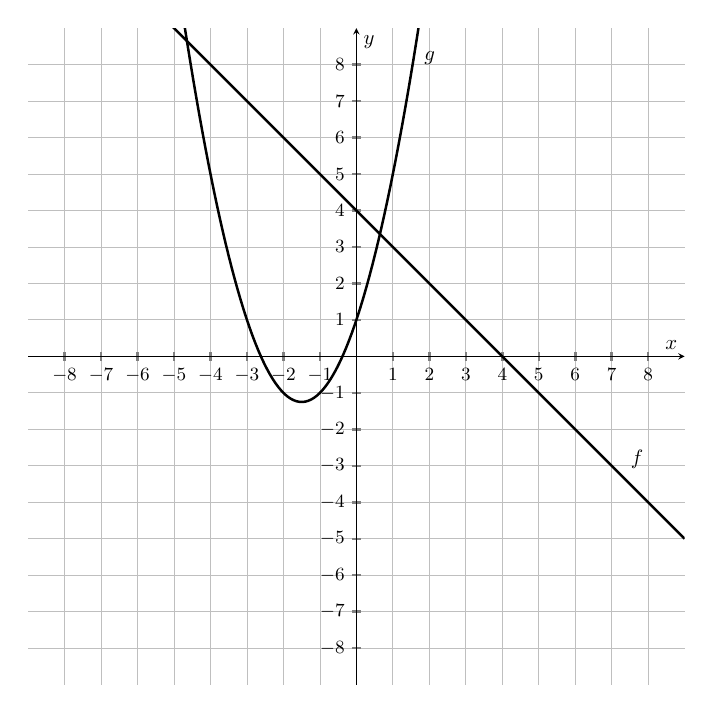
\begin{tikzpicture}[scale=0.75]
\begin{axis}[
  axis lines=center,
  grid=major,
  width=5in,
height=5in,
  xmin=-8,
  xmax=8,
  ymin=-8,
  ymax=8,
  xlabel=$x$,
  ylabel=$y$,
  enlargelimits={abs=1},
  xtick={-8,-7,...,8},
  ytick={-8,-7,...,8},
  xlabel style={at={(rel axis cs:1,0.5)}},
  ylabel style={at={(rel axis cs:0.5,1)}},
  tick style={very thick},
  ticklabel style={font=\small},
  legend style={
  at={(rel axis cs:1,1)},
  anchor=north west,
  draw=none,
  inner sep=0pt,
  fill=gray!10}
]

\addplot [very thick,domain=-8:9,samples=200] {-x+4} node [above right,pos=0.9] {$f$};
%\addlegendentry {$f(x)=...$};
\addplot[black,very thick,domain=-8:8,samples=200]{x^2+3*x+1}  node[below right,pos=0.4] {$g$};
%\addlegendentry{$g(x)=...$};
\end{axis}
\end{tikzpicture}
\end{center}	
}
\end{minipage}
\begin{boiteExT}[Quelques exemples supplémentaires]
	\vspace{7cm}
\end{boiteExT}
\end{document}


